% Copyright (c) 2005-2009 Center for Urban Simulation and Policy Analysis,
% University of Washington.  Permission is granted to copy, distribute and/or
% modify this document under the terms of the GNU Free Documentation License,
% Version 1.2 or any later version published by the Free Software Foundation;
% with no Invariant Sections, no Front-Cover Texts, and no Back-Cover Texts.
% A copy of the license is included in the section entitled "GNU Free
% Documentation License".

% This is the root latex source file for the Opus and UrbanSim Users Guide.
% The guide is organized as a set of 'include' files, normally one file
% per chapter.  It uses the Python latex documentation standards and latex
% definition files -- see http://www.python.org/doc/current/doc/doc.html
% Also see the "Writing Documentation" chapter in this manual for more
% information.


\part{The Opus Graphical User Interface}\label{part-gui}
% $Id: introduction.tex,v 1.16 2006/06/05 15:50:58 borning Exp $

\section{Introduction}

Decisions regarding major urban transportation investments, as well as
regarding policies to improve air quality and to manage urban development
to reduce the adverse effects of low-density urban sprawl, are critical,
interdependent choices that shape the long-term quality of life in urban
areas.  These choices and the problems they attempt to address have
important social, economic and environmental impacts that spill over
jurisdictional boundaries and that are impacted by decisions made by a wide
range of institutions.  In the United States, they fall into the scope of
metropolitan governance, where the institutional frameworks for forming and
implementing policy are less robust than at higher or lower levels of
government.  These metropolitan governance structures hover between the
vise-grip of local governments' control of land use decisions, and the
state and federal control of resources for transportation and environmental
regulations.  In the gap, Metropolitan Planning Organizations (MPOs) have
been created by states under federal requirements to better coordinate the
allocation of federal investments in transportation, and air quality
planning.  These MPOs generally do not have any taxing or direct
implementation or operational responsibility, but are charged with creating
regional transportation plans and coordinating these with land use and air
quality planning.  It is a tall order.

Putting institutional difficulties aside for the moment, the task of
developing regional transportation plans is complex enough at a technical
level.  How can an almost infinite list of alternative transportation
investments proposed by local governments, states, and other entities be
examined systematically and an investment plan adopted that reflects a
democratic process based on a robust assessment of the alternatives?  Over
the past several decades, MPOs and their predecessor institutions have used
simulation models to predict the volumes of traffic on the transportation
network, given assumptions about the land use patterns that would generate
patterns of travel demand on this network.  The traditional models are
called `four-step models' because they break this task into (1) predictions
of the number of trips generated and attracted in each zone of the
metropolitan area, (2) the trip distribution patterns from zone to zone,
(3) the mode choice of trips (automobile, transit, etc.)\ between
any two zones, and ultimately, (4) how
these trips are assigned to the capacity-constrained network, leading to
patterns of travel time and congestion.  These four-step models were
originally developed within the discipline of civil engineering in the late
1950's and early 1960's to address a very specific problem: how to estimate
the amount and location of additional road capacity needed to satisfy a
given demand for transportation. They became ingrained into the planning
process for transportation, reinforced by federal investment and
regulation.  In the 1960's and 1970's, the four-step travel models were
brought into mainstream use and became the mainstay analysis tool used to
support decisions on alternative road investments.

Since the 1980's, however, the models and the decision-making process have
come under increasing scrutiny and criticism, leading to substantial
pressure to revise both \cite{beimborn-1996}.  One of the central
criticisms is that the models, and the way they have been generally used,
assume that changes in land use result in different demands on the
transport system, but that changes in the transportation system do not
cause land use changes to occur.  Aside from the mountain of theoretical
and empirical evidence to the contrary, this assumption violates common
sense.  Building a major highway through farmlands cannot be expected to
have absolutely no impact on the probability that sites along the new
highway, or accessible to it, will develop.  And if there is an impact on
development, the logical extension is that it will in turn impact travel
demand.  This idea is what has been referred to as induced demand, and one
of the reasons scholars have become increasingly skeptical that it is
possible to ``build your way out of congestion'' (see \cite{downs-2004} for
example).  Since the U.S. Clean Air Act Amendments of 1990 and the Intermodal
Surface Transportation Efficiency Act of 1991, federal policy has
recognized the need to link transportation and land use, in order to
account for this relationship.  Since that time, refinement of
transportation planning practice has been slow, partly due to the technical
difficulties of accounting for the interactions, and partly due to
political constraints and the increasing role of public involvement in
decision-making processes such as these.

Early use of technology such as transportation models to support
transportation investments dates to a conception of planners as technocrats
who provide answers that are to be taken at face value and used as an
objective basis for public decisions.  Public participation in these
decisions, and in the technical analyses behind them, was decidedly not on
the agenda.  Much has changed since then, especially at the local
government level.  An increasingly sophisticated and skeptical set of
stakeholders demands public participation, as well as transparency and
access to information about the decision-making process and the assumptions
and analyses behind it.  Conflicting interests are played out in public
meeting after public meeting and in committee after committee that is
deliberating land use policies or transportation investments.
Environmental advocates have increasingly come to use the courts to prod
planning agencies to refine their analyses to address shortcomings such as
the omission of land use feedback effects \cite{garret-1996}.

%% Though the mandate for setting and managing land use policy has been
%% claimed unambiguously by local governments, the mandates for setting
%% policies that cut across local jurisdictions are much less clear.  The
%% devolution of federal responsibilities to state and local governments makes
%% the setting of these policies increasingly a metropolitan agenda, but our
%% institutional organizations at metropolitan scales are not fully developed
%% to address the these policies.  In the 1970's, a movement towards
%% regionalism spawned the creation of Councils of Governments (COG) to
%% oversee some limited aspects of coordination of local government decisions
%% and investments.  But COGs had no taxing and no real operation authority,
%% and were often criticized as being incapable of taking strong positions due
%% to their construction as agents of local governments.  Beginning around
%% 1990, federal legislation such as the Clean Air Act Amendments and ISTEA
%% began to reinvigorate metropolitan governance in the form of Metropolitan
%% Planning Organizations (MPO), charged principally with the role of
%% coordinating federal investments in transportation within their
%% metropolitan areas.  Still, these MPOs generally lack taxing and
%% operational mandates beyond coordinating long-term plans for transportation
%% investments, and have boards that are not directly elected.  Making
%% difficult decisions about the allocation of transportation funds, and the
%% even more difficult tasks of coordinating land use and environmental
%% policies with these, has generally proven to be challenging within the
%% current institutional framework for metropolitan governance.

\subsection{Urban Modeling as a Digital Government Research Area}

The domain of land use and transportation modeling thus provides an
significant opportunity for digital government research: it is of great
interest to government agencies, and it includes a set of hard, open
problems, both technical and procedural.  This chapter is intended for
digital government researchers and students who are generally computer- and
policy-literate, but who are not necessarily expert in either the domain of
urban modeling or of land use and transportation policy.  In the chapter,
we first present a taxonomy of needed refinements to urban models
themselves, and to the process of applying them.  We then present a case
study of UrbanSim, an urban modeling system that our group has been
developing at the University of Washington, including a short history, more
recent research initiatives, and some significant applications to planning
activities.

Our focus in this chapter is primarily on the U.S. context.  However,
controversies regarding land use and transportation occur world-wide, and
analogous issues arise around using models to inform decision-making in
other countries.

\subsection{A Taxonomy of Model and Process Refinements}
\label{sec:refinement-taxonomy}

Our research is intended to contribute both to improving the technical
modeling capacity to address issues such as the land use consequences of
transportation investments, as well as to improving the process of using
models in a democratic decision-making context. To help structure this case
study, as well as providing a framework for evaluating urban models, we
offer the following taxonomy of model and process refinements
(Table \ref{taxonomy-table}).  We hope
that this taxonomy will be of value beyond this particular case study as
well, for other studies of modeling and simulation in the policy arena.  In
developing this framework, we draw on and extend earlier work that has
criticized earlier urban models (for example \cite{lee-1973}).  We then
describe how our project and several research initiatives within it have
emerged to address these challenges.

\begin{table}[t]
\begin{itemize}
\item Refinement of Models
   \begin{itemize}
   \item Validity
      \begin{itemize}
      \item Accuracy
      \item Handling of uncertainty
      \item Policy sensitivity
      \end{itemize}
   \item Comprehensiveness
      \begin{itemize}
      \item Real estate development and prices
      \item Employment location
      \item Household location
      \item Transportation system
      \item Environmental impacts
      \end{itemize}
   \end{itemize}
\item Refinement of Process
   \begin{itemize}
   \item Refinement of the model construction and application process
      \begin{itemize}
      \item Feasibility of data preparation
      \item Performance
      \item Usability
      \item Support for software evolution
      \end{itemize}
   \item Support for a more effective democratic process
      \begin{itemize}
      \item Responding to stakeholder interests and concerns
      \item Transparency
      \item Fairness
      \item Facilitating stakeholder access to models and their output
      \end{itemize}
   \end{itemize}
\end{itemize}

\caption{Model and Process Refinements}
\label{taxonomy-table}
\end{table}

\subsubsection{Refinement of Models}

At the top level, we distinguish between \emph{refinement of models} and
\emph{refinement of process}.  Refinement of models focuses on the models
themselves.  In turn, we can classify the work on refinement of models
as work on \emph{validity} and on \emph{comprehensiveness}.

Validity includes improving the accuracy of the models, and also their
sensitivity to policies of interest.  Accuracy means that the predicted
values (for example, of population density in different neighborhoods) are
close to the observed values.  This raises the obvious problem of how to
evaluate the accuracy of predictions of events in the future.  One
technique is \emph{historical validation}, in which the model is run on
historical data, and the results compared with what actually transpired
(see \cite{waddell-japa-2002} for example). This has the clear merit of
comparing with real outcomes.  There are
difficulties as well, however.  First, in many cases the needed historical
data is not available.  Also, for the relatively small number of regions
for which data is available, there may not have been major land use and
transportation changes over the period being tested, so that the model in
effect isn't being used to simulate major decisions.  An alternative
technique that is
often used is to run the model system with fairly extreme scenarios
(e.g.\ doubling the capacity of selected roadways, or removing zoning
restrictions on height limits in a neighborhood).  The results are then
evaluated by an expert review panel.

Predicting the future is a risky business.  There are numerous,
complex, and interacting sources of uncertainty in urban simulations
of the sort we are developing, including uncertainty regarding
exogenous data, the model structure and specification, the
parameters of the model, and from the stochastic nature of the
simulation. Nevertheless, citizens and governments do have to make
decisions, using the best available information. Ideally we should
represent the uncertainty in our conclusions as well as possible,
both for truthfulness and as important data to assist in selecting
among alternatives.  However, to date there has been only a small
amount of work done on handling uncertainty in urban modeling in a
principled fashion \cite{sevcikova-trb-2006}.

We often also want to improve the sensitivity of the model to policies of
interest.  For example, if a region is interested in policies that foster
walkable neighborhoods, then the model should be able to model walking for
transportation as well as for health and recreation.  Which policies are of
interest is of course a political and societal question; but given such
policies, whether the model responds suitably to them becomes a question of
validity.

Yet another sort of refinement of the models is increasing their
comprehensiveness to include other actors and processes in the urban
environment.  For example, for households, we might model additional
demographic processes, such as household formation and dissolution.
Or for environmental impacts, we might model consumption of
additional kinds of resources, or the impacts of decisions on
biodiversity as well as on particular species of interest (for
example, due to Endangered Species Act considerations).

There are important pitfalls and tensions associated with the goal of
increasing the comprehensiveness of models: namely what Lee \cite{lee-1973}
called the problem of hyper-comprehensiveness.  One aspect of this is
pressure to model more and more aspects of the urban environment because
these aspects are important to someone --- even though they might have
little relation to land use and transportation.  For example, there might
be demands to model voter turnout rates.  These pressures are relatively
straightforward to deal with, by reminding stakeholders of the purpose of
the modeling work and the need to remain focused.  A more difficult issue
is that a seemingly endless number of factors influence urban land use and
transportation.  For example, crime is clearly an important factor in
residential location choice, in transportation choice, and others.  But we
need not just data on current crime rates --- and perhaps more importantly,
on people's perceptions of crime --- but also a predictive model of crime
in the future under different possible scenarios.  This is both difficult
and controversial.  For example, what are the major determinants of the
crime rate?  Economic conditions?  Family stability and moral instruction?
The nature of the criminal justice system?  How far should the modeler go
down this path?  Or as another example (relevant to the region around
Seattle), suppose we want to model the return rate of wild salmon in rivers
and streams that flow through urban regions.  There are many factors
affecting this: the amount of impervious surface, pollutants from
agricultural runoff, the number of fish caught by both commercial and sport
fishers, oceanic conditions (including temperature, since the salmon grow
to maturity in the ocean before returning to fresh water streams to spawn),
and many others.  Among the pitfalls of overly ambitious modeling are
increasing model complexity, additional data requirements, and in some
cases the credibility of the overall modeling effort.

\subsubsection{Refinement of Process}

Returning to the top level of the taxonomy, refinement of process includes
first, improving the process of developing, extending, and applying models;
and second, supporting their more effective use in a democratic society.
The first of these is concerned with instrumental values such as usability
and feasibility: data preparation issues, adequate performance, usability
of the software, and accommodating changes in requirements, data, and the
like.  It must be feasible to prepare the data needed to run the model.
Typically, this implies that the data must already be in hand ---
collecting new data is enormously expensive.  But the data in hand may be
of varying quality, or in the wrong format, and so forth.  Performance should
be adequate, and the software must be usable by the technical staff at the
planning organization.  Also, the model system architecture should allow
for the system to evolve as requirements and the questions asked change
over time.

Another set of process issues revolve around the desire to use modeling as
part of a more participatory, open, and democratic process, rather than in
a technical, back-room exercise.  One aspect of this is improving the
relevance of the modeling and output to the diverse range of stakeholder
concerns (in other words, increasing its comprehensiveness in response to
stakeholder values).  Transparency of the model itself, of the input data
preparation process, and of the overall context in which it is used also
play an important role as well.  Another aspect of this is improving the
fairness of the model (for example, in not omitting an important
transportation mode, or short-changing the interests of renters as compared
with home owners).  Again, this can result in additional demands for
refinement of the model (either its validity, comprehensiveness, or both).
The results of running the model, and ideally even the ability to
experiment with alternatives, should be opened up to a wider range of
stakeholders, rather than being restricted to the technical modelers.
System performance is relevant here also: for example, if the model takes
weeks to run, clearly this would make it difficult to use to support
deliberation, in which model results are discussed, and in response new
questions are asked of the model or new scenarios are proposed for testing.

There are some obvious tensions among these objectives for refinement of
models and process.  Pressures to increase policy sensitivity in order to
avoid bias from omission of certain policies from consideration, for example
pedestrian and bicycling modes, increase the need for
a very high level of behavioral and spatial detail.  This
will certainly come at a cost in performance, and
quite possibly also at a cost of some reduction in the accuracy of the
results.  How can model sensitivity, data requirements, transparency,
computing performance, and accuracy be compared against each other?  How are
the interests of different stakeholders served by alternative compromises
among these?  How do these choices affect the legitimacy of the model
system and the process for using it in the decision-making process?  These
are difficult problems, and ones that have not received sufficient
attention to date.  We seek to address these concerns in our project in
addition to the more purely technical issues of model refinement.

% LocalWords:  borning MPOs Intermodal analyses UrbanSim pwaddell

\chapter{The Variable Library}

The variable library is a repository for variables defined in the system.  These variables can be used generally throughout the system, whether for defining variables to help predict property values or household location choices, or to compute indicators that are useful for evaluating simulation results, like change in open space or in population density.  Since it provides a resource that is used throughout the GUI, we access it from the tools menu on the menu bar at the top of the main window, as in Figure \ref{fig:variable-library-menu}.  The screenshot in Figure \ref{fig:variable-library-main} shows a popup window that appears once a user selects the variable library option on the tools menu.  Note that the contents of it depend on what project is loaded.  In this case, we have the eugene\_parcel project loaded, and see the variables that are initially available.  

\begin{figure}[htp]
\begin{center}
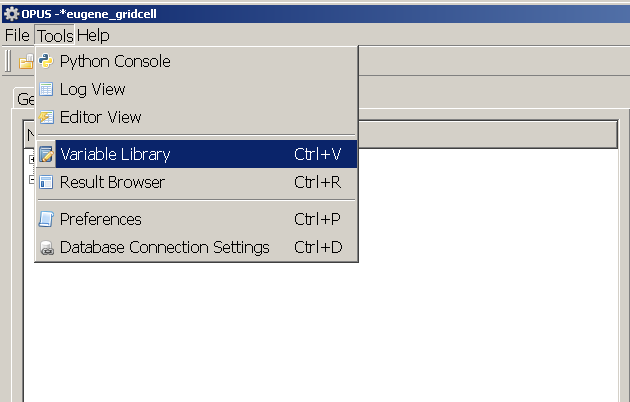
\includegraphics[scale=0.6]{part-gui/images/model-manager-variable-library-menu.png}
\end{center}
\caption{Variable Library Menu}
\label{fig:variable-library-menu}
\end{figure}

\begin{figure}[htp]
\begin{center}
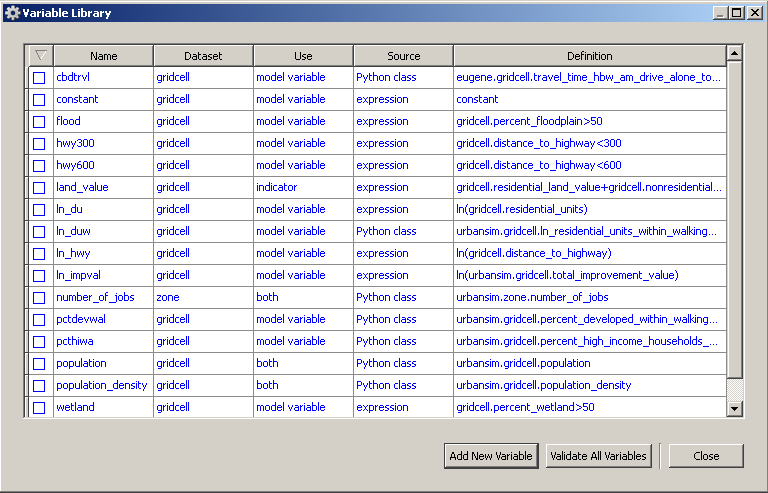
\includegraphics[scale=0.6]{part-gui/images/model-manager-variable-library-main.png}
\end{center}
\caption{Variable Library Main Window}
\label{fig:variable-library-main}
\end{figure}

Note the buttons at the bottom of this window to add new variables or validate all variables.  Adding a new variable is straightforward, using the GUI and the OPUS expression language, which provides a simple syntax for defining variables.  Notice examples of these in the variable library window, in the right-most column.  Expressions are simply functions of one or more primary attributes (think of these as columns in the input database) and possibly functions of other expressions as well.  For example, the expression for wetland is defined as gridcell.percent_wetland>50.  This defines the creation of a true/false, or boolean, variable that is interpreted as 1 if the gridcell has more than 50 percent coverage by wetland, 0 otherwise. Chapter \ref{chap:creating-variables} provides a more thorough introduction to the use of expressions and variables.

If you click on the add new variable button at the bottom of the variable library window, it opens a dialog box as shown in Figure \ref{fig:new-variable}.  The top entry is the name you want to use for the variable.  Let's say we want to create a new variable that is a log of population density.  We already have a population density variable defined by gridcell, so we can just take the log of this value.  Let's name the variable ln\_population\_density, leave the middle selection as \emph{expression}, and fill in a simple expression in the definition area: \emph{ln(gridcell.population_density)}.  Note that the dialog box provides two buttons to help you check your new variable.  The check syntax button tests whether the expression you have entered passes the Python and expression syntax checkers -- in other words, is it syntactically correct.  The second allows you to test whether if you apply this expression to your available data, it can successfully compute a result.  This is very helpful in determining whether you might have referred to a data element that is not present, or is otherwise not computable with your data.  In short, these two tools allow thoroughly testing whether the variables are in a state that can be computed on the available data.

\begin{figure}[htp]
\begin{center}
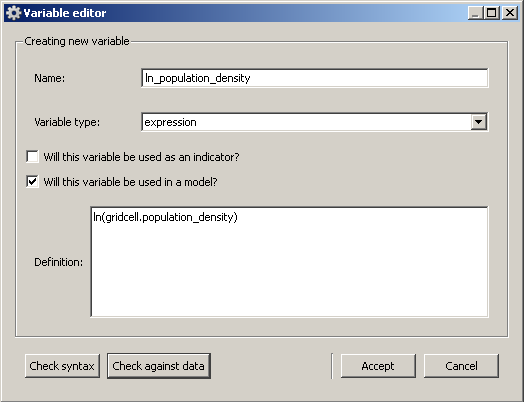
\includegraphics[scale=0.6]{part-gui/images/model-manager-variable-library-new-variable.png}
\end{center}
\caption{Adding a New Variable}
\label{fig:variable-library-new-variable}
\end{figure}
\chapter{The Menu Bar}

The main menu bar at the top of the OPUS GUI main window has three dropdown
menus: File, Tools, and Help.  The File menu includes the standard
operations of opening a project, saving a project, saving a project under a
new name, closing an OPUS Project, and finally exiting the OPUS GUI\@.  Help
offers an About option which produces a dialog box with information about
OPUS and a set of links to the UrbanSim website, online documentation, and
the GNU License.  The Tools menu provides access to several general tools,
described below.

Most of the items in the main menu bar are accessible from a secondary menu
bar just above the tabs on the left side of the OPUS GUI window.  Hovering
over each icon will yield a tooltip with the item's description.

\section{Tools}

The Tools menu, shown in figure \ref{fig:menu-bar-tools}, enables users to
adjust settings and preferences, as well as opening different tabs in the
right set of tabs.  The items labeled ``Python Console'', ``Log View'', ``Editor
View'', and ``Result Browser'' will each open new tabs on the right.  The
Result Browser is covered in greater detail in section
\ref{sec:interactive-result-exploration}.  The items labeled ``Variable
Library'', ``Preferences'', and ``Database Connection Settings'' each open a
popup when clicked.  The Variable Library is further discussed in section
\ref{chap:variable-library}.

\begin{figure}[htp]
\begin{center}
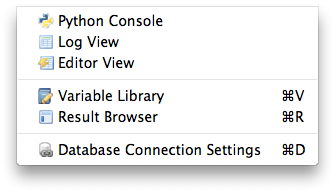
\includegraphics[scale=0.4]{part-gui/images/menu-bar-tools.png}
\end{center}
\caption{Tools Menu}
\label{fig:menu-bar-tools}
\end{figure}


\section{Preferences}

The Preferences dialog box changes some user interface related options in
the OPUS UI.  The dialog box is split into two sections, font preferences
and previous project preferences.  The font preferences section allows
users to adjust font sizes specific to different areas of the GUI.  The
previous project preferences section contains a checkbox allowing users to
open the most recently opened project each time OPUS GUI is started, this
is turned off by default.  Changes to the user preferences take effect as
soon as either the ``Apply'' or ``OK'' buttons are clicked.

\section{Database Server Connections}\label{sec:database-server-connections}

Database connections can be configured in the Database Server Connections
dialog launched from the Tools menu.  The Database Server Connections
dialog, pictured in Figure \ref{fig:menu-bar-database-connections}, holds
connection information for four database servers.  Each connection is used
for a specific purpose.  While there are four different connections that
must be configured, each may be configured to use the same host.  Every
connection requires a protocol, host name, user name, and password to be
entered.  Editing the protocol field produces a drop down of database
protocols that UrbanSim is able to use.  If a server has been setup for
UrbanSim's use choose the protocol that corresponds to the type of SQL
server being used.  If no SQL server is setup for a particular use, SQLite
may be used.  SQLite will create a local flat-file database instead of a
remote server.  UrbanSim currently supports MySQL, Microsoft SQL Server,
Postgres, and SQLite.

The Database Connection Settings are saved when the Accept Changes button
is pressed, ensuring that all future database connections will be made
using the new settings.  Database connections that are still in use while
the database connection settings are being edited will not be changed until
the connection is reestablished, for this reason it may be necessary to
reopen any open project after changing the database connection settings.

\begin{figure}[htp]
\begin{center}
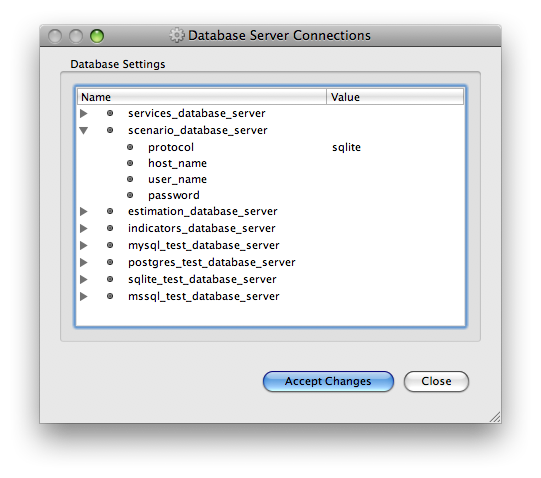
\includegraphics[scale=0.6]{part-gui/images/menu-bar-database-connections.png}
\end{center}
\caption{Database Connections}
\label{fig:menu-bar-database-connections}
\end{figure}

\chapter{General}

\chapter{The Data Manager}
The Data Manager\index{Data Manager} has two primary purposes, each reflected in the sub-tabs.  One tab, the Opus Data 
tab\index{Opus Data tab}, is for browsing, viewing, and exporting data from the Opus data cache.  
The other tab, the Tools tab\index{Tools tab}, is a place for storing and executing various tools provided by the Opus community or tools you have written.

\section{Opus Data Tab}

The Opus Data tab is a file browser that defaults to the folder in which
your project creates data.  This folder name is composed from the default 
location for the Opus files, followed by \file{data}, followed by the project
name.  The project name for the \file{eugene_gridcell_default.xml} project is
``eugene\_gridcell.'' (This is given in the ``project\_name'' element in the xml.)
Thus, if you installed to
\file{c:/opus}, and you are opening the Eugene sample project at
\file{c:/opus/project_configs/eugene_gridcell_default.xml}, the data folder
for this project is \file{c:/opus/data/eugene_gridcell}.  That is the
folder that this view starts at.  Any subfolders and files are displayed in
the tree view.  See Figure \ref{fig:opusdatatab}.

\begin{figure}[htp]
\begin{center}
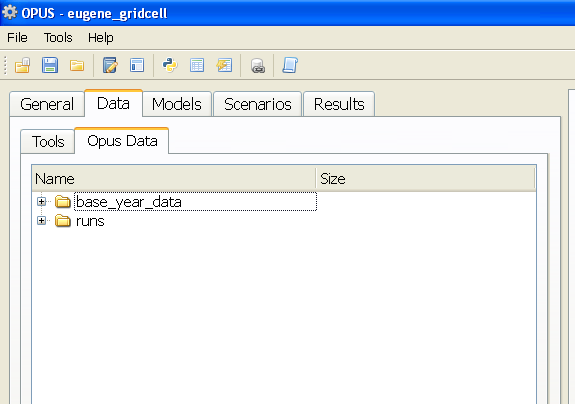
\includegraphics[scale=0.6]{part-gui/images/data-manager-opus-data-tab.png}
\end{center}
\caption{The Opus Data Tab}
\label{fig:opusdatatab}
\end{figure}

There could be any number of subfolders here, but by default you will find
a \file{base_year_data} folder\index{base\_year\_data}, and a \file{runs} folder\index{runs folder}.  The
base_year_data folder will normally contain an Opus \file{database} folder.
An Opus database folder\index{Opus database folder} is any folder containing Opus \file{datasets}.
Often Opus database folders are titled with a year, such as 2000.  Opus
datasets are folders containing Opus `data arrays.'  Opus datasets are
equivalent to the tables in a database.  Opus data arrays are equivalent to
the columns in a table, and are simply numpy arrays that have been written
to disk in a binary format.  See Figure \ref{fig:db-dataset-array}.

\begin{figure}[htp]
\begin{center}
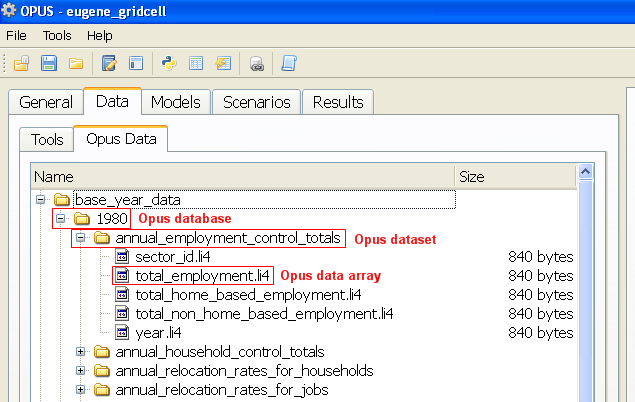
\includegraphics[scale=0.6]{part-gui/images/data-manager-opus-data-tab-db-dataset-array.png}
\end{center}
\caption{Opus databases, datasets, and arrays}
\label{fig:db-dataset-array}
\end{figure}

The Opus data arrays are referred to throughout the documentation as
`primary attributes.'  Primary attributes are the actual data columns in a
dataset.  Computed attributes are attributes computed from primary
attributes via expressions.  For instance, if a parcels dataset contained
the primary attributes population and area, a computed attribute called
population_density could be computed by using the expression
\variable{population_density = population/area}.  Once this expression is
entered and stored in your project in the Variable Library, it can be used
in a model and would be computed as needed.  See Chapter~\ref{chapter:expressions} 
for more details on expressions.

\subsection{Viewing and Browsing an Opus Data table}
To view and browse the contents of an Opus dataset, right-click a data table, then select 'View Dataset'.  This will bring up a new tab on the right-hand side of the Opus GUI window that will display some summary statistics about the dataset, and a table view of the raw data that can be browsed and sorted by clicking the column name.  See Figure \ref{view-and-browse} for an example of browsing a data table.

\begin{figure}[htp]
\begin{center}
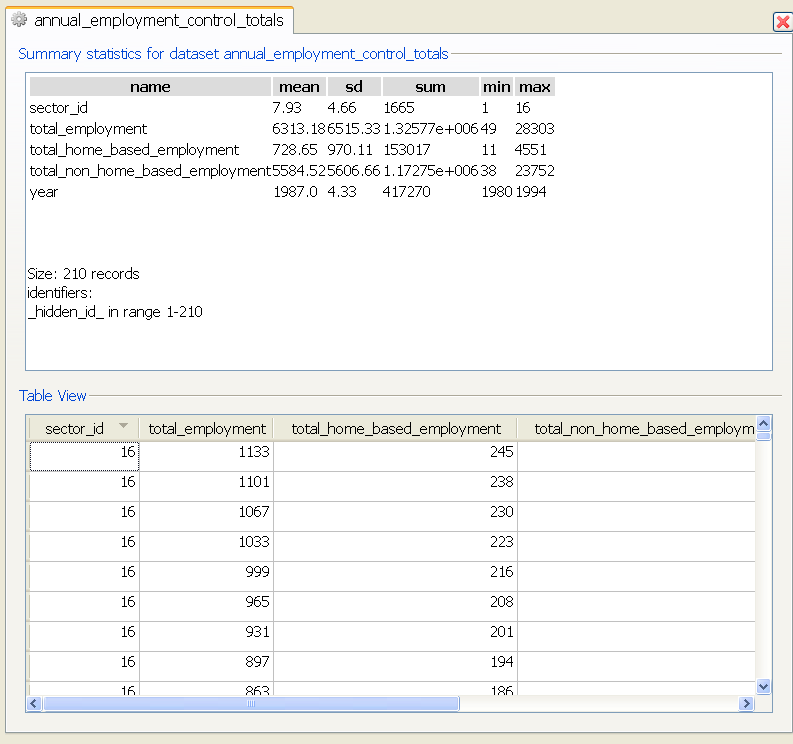
\includegraphics[scale=0.5]{part-gui/images/data-manager-opus-data-tab-view-dataset-tab.png}
\end{center}
\caption{Viewing and browsing an Opus dataset}
\label{view-and-browse}
\end{figure}

\subsection{Exporting an Opus Data table}
An Opus dataset can be exported to another format for use in other applications.  By default there are 3 options: ESRI, SQL, and CSV.  To export a dataset, right-click a dataset, choose 'Export Opus dataset to,' then click your choice.  See Figure \ref{exporting} for the right-click menu.  You will then see a pop-up window with the respective export tool with the parameters partially filled in based on which dataset you clicked.  These are the same tools that you will find in the Tools tab of the Data Manager.  For more information on the individual tools see the help tab on each tool.

\begin{figure}[htp]
\begin{center}
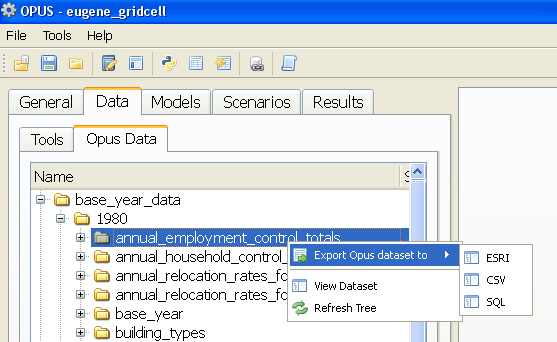
\includegraphics[scale=0.8]{part-gui/images/data-manager-opus-data-tab-export-dataset.png}
\end{center}
\caption{Exporting an Opus dataset}
\label{exporting}
\end{figure}

\section{Tools Tab}
The Tools tab\index{Tools tab} is an area to collect and execute tools and batches of tools provided with the interface, or it can be extended with tools that you  write.  A Tool is simply any script that is written in Python and executed by the interface.

\subsection{Tool Library}
The Tool Library\index{Tool library} is a place to collect and organize your tools.  Tools can also be executed directly from the library in a 'one-off' manner, meaning that you can supply parameters to the tool and execute it without storing those parameters for future use.  To execute a tool from the library, simply right-click it and choose 'Execute Tool...', see Figure \ref{execute-tool}.  This will pop-up a window in which you can supply parameters to the tool then execute it.

\begin{figure}[htp]
\begin{center}
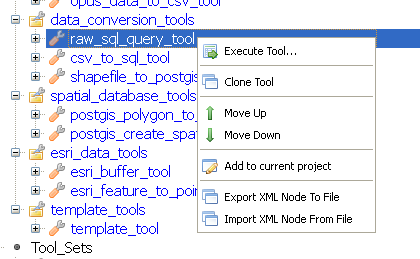
\includegraphics[scale=0.8]{part-gui/images/data-manager-opus-tools-tab-execute-tool.png}
\end{center}
\caption{Executing a tool}
\label{execute-tool}
\end{figure}

\subsubsection{Extending the Tool Library}
New tools can be written and added to the tool library fairly easily.  The best way to explain this is to use an example.  A 'template_tool' has been provided so you can see how it works.  Feel free to execute the template_tool, it just implements a simple loop and prints the results to the tool's log window.  The template_tool's code and associated XML display everything that is needed to add a tool to the interface.  See the code in the source code tree at /opus_gui/data_manager/run/tools/template_tool.py.  A tool also needs XML configuration data in an Opus project.  To view the XML configuration data for the template_tool, open urbansim.xml in an XML editor from the source code tree at /urbansim/configs and search for template_tool.

At the time of this writing new tools must be placed in the source tree at /opus_gui/data_manager/run/tools in order to run correctly.  There are plans to create an additional 'user tools' folder where tools could also be placed.  Also, at this moment, the XML must be hand written to ensure that the tools show up properly in the interface and execute correctly.  There are some right-click functions in the Tool Library to assist with the XML editing (to add a new tool, create parameters for it, etc.) but these functions are in a beta state.

Once a new tool and its associated XML is written properly, the Tool Library will display the tool and dynamically populate the pop-up dialog box with the proper parameters based on the XML configuration.  The tools are quite flexible.  Although the initial tool must be written using Python, there is no limit placed upon what one can do.  For starters, there are tools provided in the interface that make OS calls to external executables (e.g. ogr2ogr.exe), databases, and myriad other libraries to accomplish various tasks (e.g. ESRI geoprocessing).  Feel free to browse the source code for any provided tool along with the XML configuration to see some possibilities.

\subsection{Tool Sets}
Tool Sets are simply collections of tools from the Tool Library with parameters stored so they can be executed repeatedly or in order in a batch manner.  Tool Sets can contain any number of tools from the Library.  A new Tool Set can be created by right-clicking Tool_Sets and choosing 'Add new tool set.'  This adds a new Tool Set to the bottom of the list.  It can be renamed by double-clicking it and typing in a name, taking care to not use spaces or a leading integer as these are invalid in XML nodes.  Once you have a new Tool Set, tools from the Library can be added to it by right-clicking a Tool Set and choosing 'Add Tool to Tool set.'  See Figure \ref{addtool} for an example of what this looks like.

\begin{figure}[htp]
\begin{center}
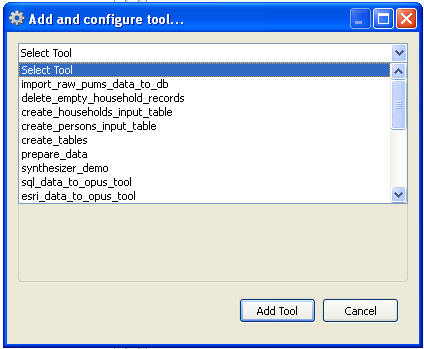
\includegraphics[scale=0.8]{part-gui/images/data-manager-opus-tools-tab-add-tool-to-tool-set.png}
\end{center}
\caption{Adding a tool to a Tool Set}
\label{addtool}
\end{figure}

From this window, choose a tool from the drop down menu, fill in the parameters, then click 'Add Tool.'  The tool is added to the Tool Set and the parameters you entered are stored in the project XML file.  This configured tool can now be executed by itself with those parameters, or executed as part of a batch in the Tool Set.  Tools in a Tool Set can be re-ordered by right-clicking them and choosing to move them up or down, and all of the tools can be executed in the order they appear by right-clicking a Tool Set and choosing 'Execute Tool Set'.

\chapter{The Models Manager}

The model manager tab\index{Model Manager tab} in the GUI provides the functionality to create models of various types, configure them, specify the variables to use in them, and then estimate their parameters if they have a form that needs to be estimated -- such as regression models or discrete choice models.  A more thorough description of the types of models that can be implemented in OPUS is provided in Chapter \ref{chap:creating-models}.

\begin{figure}[htp]
\begin{center}
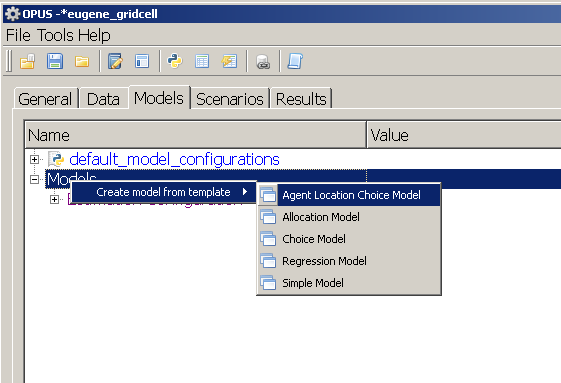
\includegraphics[scale=0.6]{part-gui/images/model-manager-create-model-from-template.png}
\end{center}
\caption{Creating a New Model from a Template}
\label{fig:create-model}
\end{figure}

\section{Creating an Allocation Model}

To demonstrate the process of creating models\index{creating an Allocation Model} in the GUI, let's begin with a simple allocation model, which does not have any parameters to estimate and represents a straightforward model to configure.  Say we want to create a model that allocates home-based jobs to zones, and lack sufficient data to specify a choice model or regression model for this purpose.  Home-based jobs are those jobs that are located in properties that are residential in character.  Assume that we have no behavioral information about this problem, other than the insight that home-based jobs are... home-based.  So we can infer that we should probably allocate these jobs to places that have housing (or households).  In allocating these jobs to zones (traffic analysis zones used in the travel model), we can count how many residential units are in each zone, and use this as the weight to allocate the total home-based jobs to zones.  That is, we want to proportionately allocate home-based jobs to zones, weighted by the number of residential units in the zone.  This is equivalent to saying that we want each residential unit to have an equal probability of receiving a home-based job (assuming that we do not have any information to suggest which residential units would be more likely than others to receive such a job).

The next consideration is the capacity of zones to absorb home-based jobs.  One simplifying assumption we could make is that there is a maximum of one home-based job per residential unit in a zone.  On average, our aggregate information suggests that most residential units do not have a home-based job, so this assumtion should not be constraining.

We now have all the information we need to specify a model for home-based jobs.  We will name the model allocate\_home\_based\_jobs, to be descriptive.  The table below contains the \emph{arguments} we will need to use in creating this model in the GUI.

\begin{table}[htp]
\caption{Creating an Allocate Home Based Jobs Model}
\label{tab:allocation-model}
\begin{center}
\begin{tabular}{ p{1.5in}  p{4.4in}  }
\toprule[1.5pt]
Configuration Entry & Value \\
\midrule
Model Name & allocate\_home\_based\_jobs\_model \\
Dataset & zone \\
Outcome Attribute & home\_based\_jobs \\
Weight Attribute & zone.aggregate(building.residential\_units) \\
Control Totals & annual\_employment\_control\_totals \\
Year Attribute & year \\
Capacity Attribute & zone.aggregate(building.residential\_units) \\
\bottomrule
\end{tabular}
\end{center}
\end{table}

The create new model dialog box (Figure {fig:create-model}) contains several kinds of model templates we could create a model from. One of these is Allocation Model. The capacity to create new allocation models, such as this, is now available in the Opus GUI. Select Allocation Model from the list, and a new dialog box appears, with several fields to fill in.  Fill in the fields with the contents from Table \ref{tab:allocation-model}, and save it.  Once this is done, it will appear in the list of models under the Models section of the Model Manager tab.  It is now a fully enabled model, and can be included in a simulation run.

It should go without saying (but doesn't), that creating models through the GUI, with a few mouse clicks and filling in a few fields in a dialog box, is much, much easier than it has been in the past. One does not need to be an expert software developer in order to create and use interesting and fully functional models in OPUS.


\begin{figure}[htp]
\begin{center}
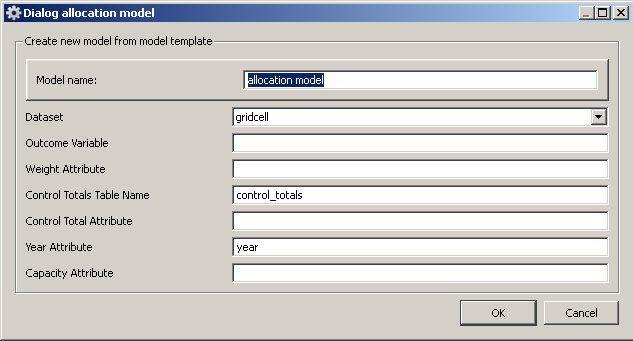
\includegraphics[scale=0.6]{part-gui/images/model-manager-create-allocation-model-from-template.png}
\end{center}
\caption{Creating a New Allocation Model from a Template\index{creating an Allocation Model}}
\label{fig:create-allocation-model}
\end{figure}

\section{Creating a Regression Model}

Regression models\index{creating a Regression model} are also simple to create and specify in the Opus GUI, and can be estimated and simulated within the graphical interface.    Assume we want to create a model that predicts population density, using the population per gridcell as the dependent variable and other attributes we can observe about gridcells as independent (predictor) variables.  Note that this is not a very useful model in this context since we actually have a household location choice model to assign households to gridcells -- so this model is for demonstration purposes only.

To create this model in the Opus GUI, right-click again on Models, and select in this case Regression Model to generate a new dialog box for this model template, as shown in Figure \ref{fig:create-regression-model}.  We just need to provide three arguments in the dialog box - a name to assign to the new model (we will use population\_density\_model), a dataset to contain the dependent variable (gridcell), and the name of the dependent variable (population\_density) - which should exist in the base year, or be an expression to compute it from other attributes already in the data.


\begin{figure}[htp]
\begin{center}
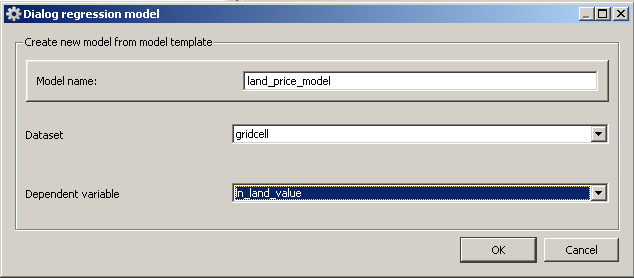
\includegraphics[scale=0.6]{part-gui/images/model-manager-create-regression-model-from-template.png}
\end{center}
\caption{Creating a New Regression Model from a Template\index{creating a Regression model}}
\label{fig:create-regression-model}
\end{figure}

Once the values have been assigned to the configuration of the new model, and you click OK on the dialog box, the model is added to the list of models under Models.  If you expand this node by clicking on the plus sign to the left of the new land price model entry, you will see that it contains a specification and a structure node.  Expand the specification node, and you will find some additional detail, including a reference to submodels, and a variables entry.  We will ignore submodels for now -- it is a means of specifying that you would like to specify the model differently for different subsets of the data.  For now we will just apply a single specification to all the data, to keep this a bit simpler.  We can now move to the task of specifying and estimating this model. 

Right-click on the variables node, and click on Select Variables, as shown in Figure \ref{fig:specify-regression-1}.  At this point a window should appear as shown in Figure \ref{fig:specify-regression-2} that is essentially the same as the variables library window you encountered earlier.  There is a column of check-boxes at the left hand side of the window which you can use to identify the variables you want to include as independent variables, or predictive variables, for this model.  The button at the bottom allows you to accept the selection, which then updates the list of variables in the model specification.  Try adding a constant term, since this is a regression and we need an intercept, or a base value.  Also add a variable like population density.  Now accept the selections.


\begin{figure}[htp]
\begin{center}
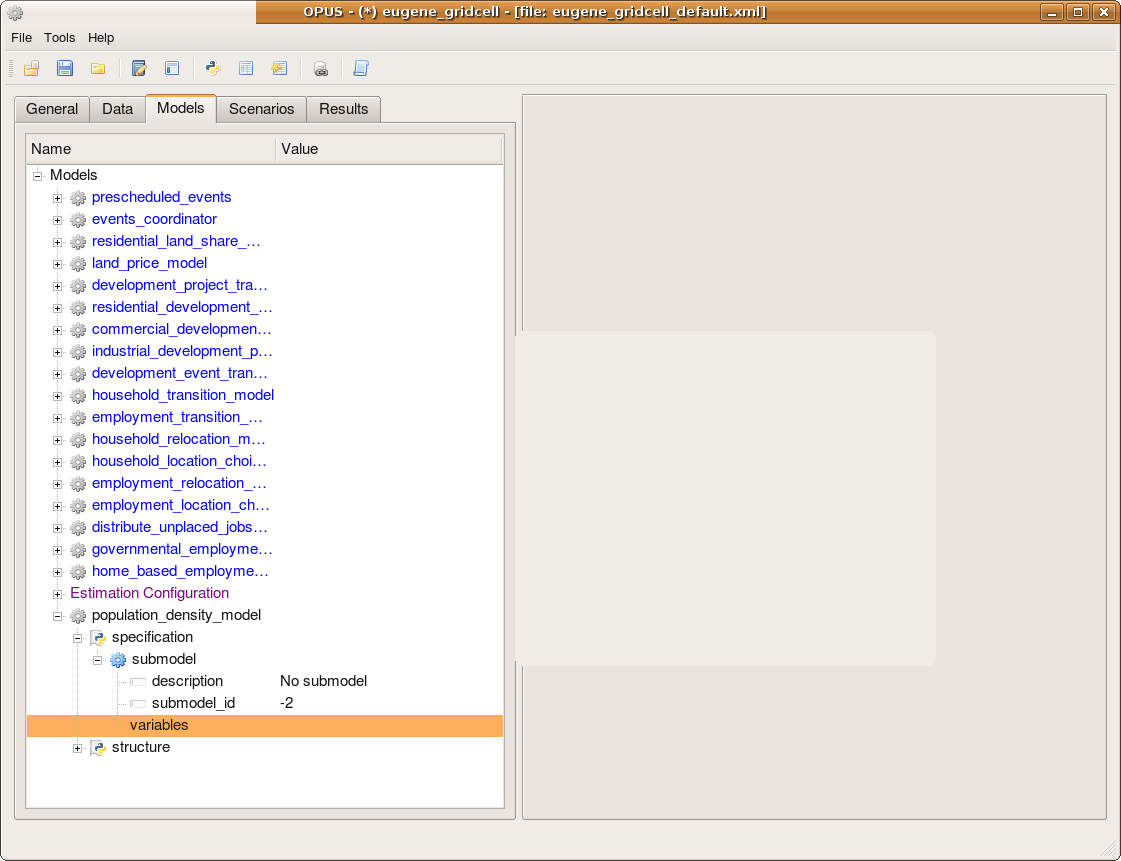
\includegraphics[scale=0.4]{part-gui/images/model-manager-specify-regression-model-1.png}
\end{center}
\caption{Specify the New Population Density Model}
\label{fig:specify-regression-1}
\end{figure}

\begin{figure}[htp]
\begin{center}
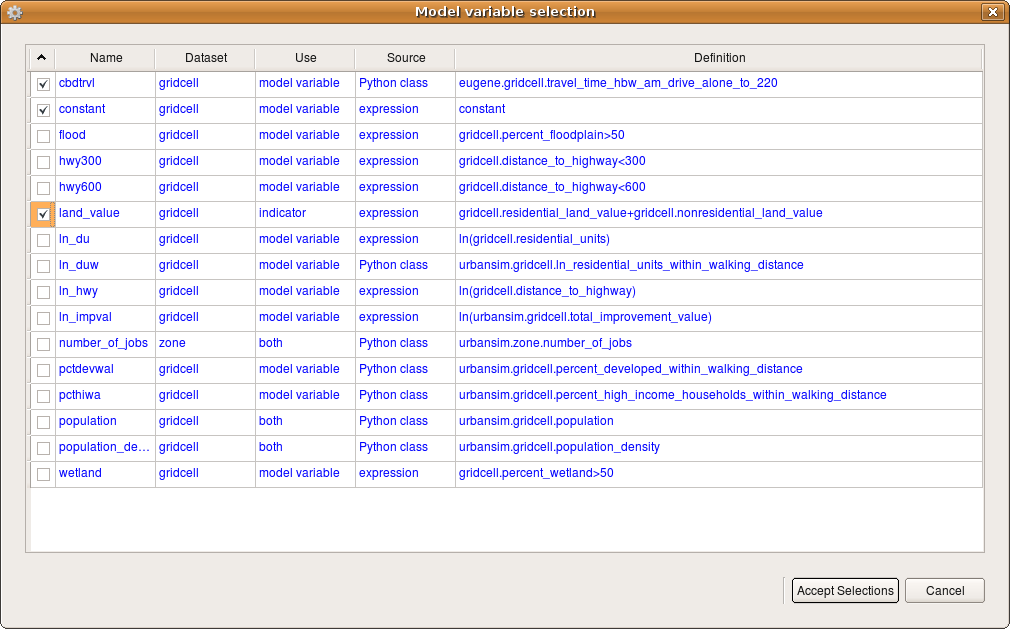
\includegraphics[scale=0.4]{part-gui/images/model-manager-specify-regression-model-2.png}
\end{center}
\caption{Select Variables for Specification}
\label{fig:specify-regression-2}
\end{figure}


Once the model specification has been entered, we can estimate the model parameters using Ordinary Least Squares by right-clicking on the population density model and selecting Run Estimation, as shown in Figure \ref{fig:specify-regression-3}. Once this has been clicked, a new tab appears on the right hand side of the main window, to interact with the model estimation.  Click on the start estimation button, and within a few seconds you should see the estimation results appear in this tab, as shown in Figure \ref{fig:specify-regression-4}.

\begin{figure}[htp]
\begin{center}
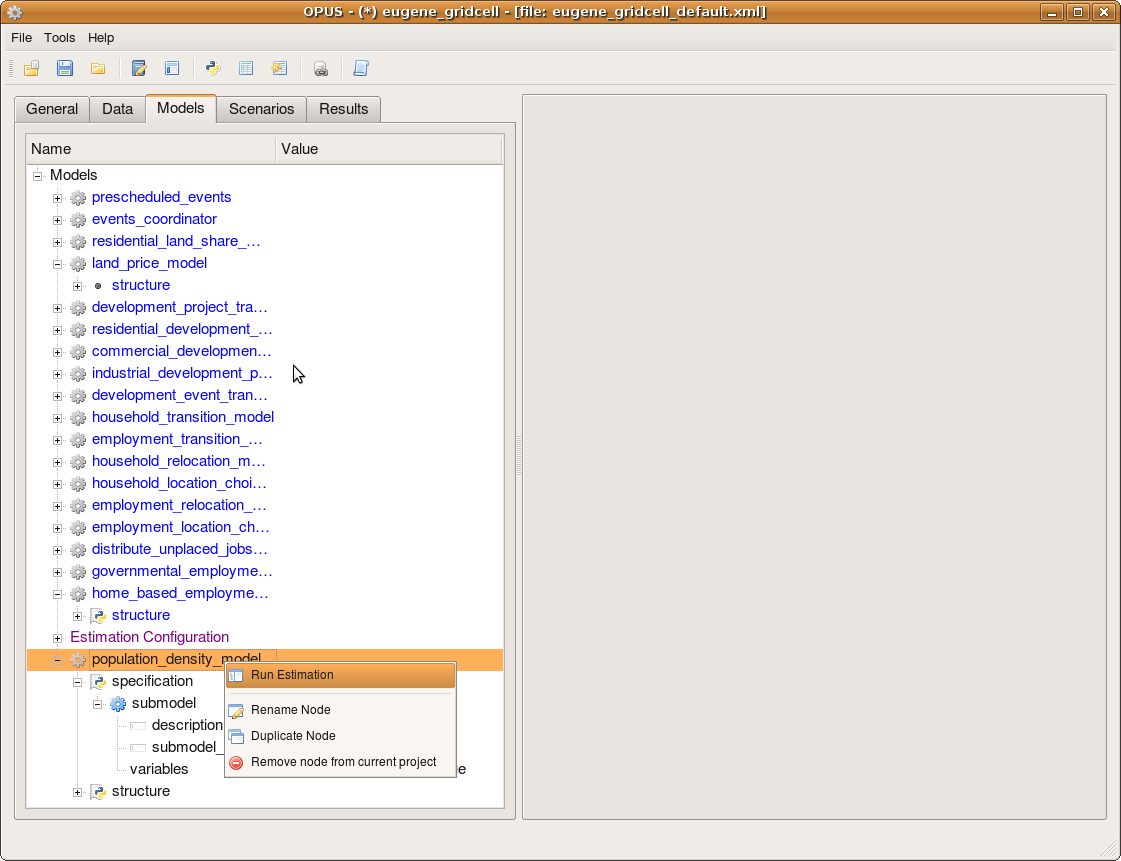
\includegraphics[scale=0.4]{part-gui/images/model-manager-specify-regression-model-3.png}
\end{center}
\caption{Estimate the New Population Density Model}
\label{fig:specify-regression-3}
\end{figure}

\begin{figure}[htp]
\begin{center}
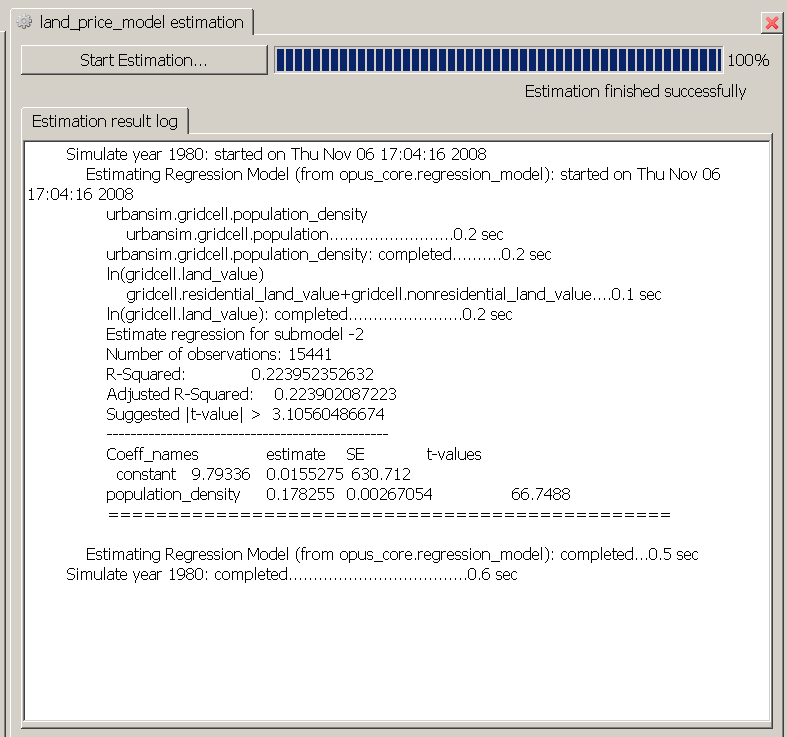
\includegraphics[scale=0.4]{part-gui/images/model-manager-specify-regression-model-4.png}
\end{center}
\caption{Estimation Results}
\label{fig:specify-regression-4}
\end{figure}

We can see from the results that the constant and travel time to the CBD, and also land value were quite statistically significant, and that they explain around 28 percent of the variation in population density in Eugene.  Clearly this is a toy model, but adding other variables in this way can increase the explanatory power to a quite useful level, and as you can see modifying the specification and estimating the model is not difficult to do.

One other note at this point is that the specification and estimation results are automatically stored, if you request this, as shown in Figure  \ref{fig:save-estimation}.  Once the estimation is done, then, the model is ready to use in a simulation, or predictive mode.  More on this in the Scenario Manager section.

\begin{figure}[htp]
\begin{center}
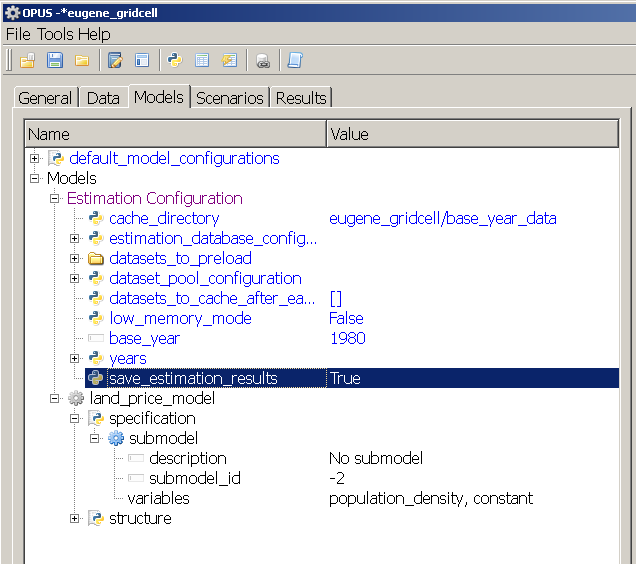
\includegraphics[scale=0.6]{part-gui/images/model-manager-save-estimation.png}
\end{center}
\caption{Save Estimation Results Flag}
\label{fig:save-estimation}
\end{figure}


%\section{Creating a Choice Model}
% Replace this later, after further testing and cleanup
%The next type of model we will create is a choice model.  This is a very common modeling application, and is used widely.  Our example for this demonstration is a model of housing type choice, which for purposes of keeping the example simple, we reduce to two alternatives: single-family housing type, or other.  It is likely that households choosing to live in single-family housing may make different trade-offs in other choices, such as travel, and car ownership.  By reducing the model to two outcomes, we create a binary choice model specification.  We always need to use one alternative as a base of comparison in choice models, so for this model we will use the other housing type as the base of comparison.  

%Below are the configuration settings for creating a choice model of housing type.  In order to create this model for estimation purposes, we will exclude the few households that are in non-residential property types, and only keep those in multi-family, condominium, and single-family housing.  These are reflected by building type id values of 4, 12, and 19, respectively, in the seattle parcel data.  Filtering the data to include only these three values can be done with the numpy logical\_or command, but since it takes only two arguments, we need to create a nested comparison, as shown below.  Since there are three housing types represented in this data, and we want to create a binary choice outcome for simplicity, it is necessary to create a dependent variable that is 2 if the household occupies a single family house, and 1 otherwise.  In this example, since we will use the entire household table, we draw a small sample of 5\% of the agents to use in estimating the model.

%\begin{table}[htp]
%\caption{Creating a Housing Type Choice Model}
%\label{tab:housing-type-choice-model}
%\begin{center}
%\begin{tabular}{ p{1.2in}  p{1.2in} p{3.2in}  }
%\toprule[1.5pt]
%Configuration Entry & Node & Value \\
%\midrule
%Model Name & & housing\_type\_choice\_model \\
%Choice Set & Init & [1, 2] \\
%Choice Attribute & Init & single\_family=(household.disaggregate\\ & & (building.building\_type\_id)==19)+1 \\
%Estimation Size Agents & Init.Estimation Config & 0.05 \\
%Agent Set & Run, Prepare for Run, Estimate, Prepare for Estimate & household \\
%Agent Filter & Prepare for Run & numpy.logical\_or(numpy.logical\_or(household.\\ & & %disaggregate(building.building\_type\_id)==4,household. \\ & & disaggregate(building.building\_type\_id)==12),household.\\ & & %disaggregate(building.building\_type\_id)==19) \\
%Specification Table & Prepare for Run & housing\_type\_choice\_model\_specifications \\
%Coefficients Table & Prepare for Run, Prepare for Estimate & housing\_type\_choice\_model\_coefficients \\
%\bottomrule
%\end{tabular}
%\end{center}
%\end{table}

%Figure \ref{fig:configure-choice-model} shows the housing type choice model configuration in progress.  For a binary choice model such as this, the specification of the model is quite similar to the specification of the regression model, but there are some subtle differences.  The most important one is that, as this model is implemented in Opus now, it requires at least one variable in each equation - that is - per alternative.  We typically assign the constant to alternative 1, and all other variables to alternative 2.  In a future revision of the code, the base alternative will not take any variables (this is the more standard implementation).  Figure \ref{fig:choice-model-specification} shows the initial specification of the housing type choice model, with a constant for the other housing types, and income and has\_children included in the utility specification for the single family housing alternative. 

%Once the model is specified, it needs to be added to the list of models to estimate, and selected as the model to estimate, as was the case in the preceding regression model example.  Once the model has been added and the project saved, the model can be estimated with the normal right-click option on the models to estimate node.  The results are shown in Figure \ref{fig:choice-model-estimation}.

%\begin{figure}[htp]
%\begin{center}
%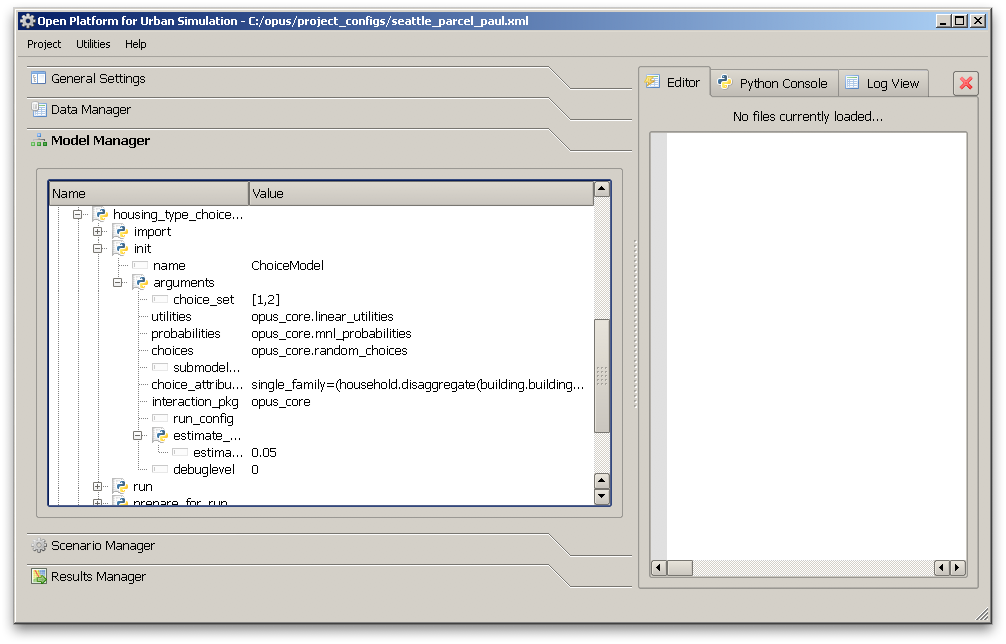
\includegraphics[scale=0.35]{graphics/configure-choice-model.png}
%\end{center}
%\caption{Configuring the Housing Type Choice Model}
%\label{fig:configure-choice-model}
%\end{figure}

%\begin{figure}[htp]
%\begin{center}
%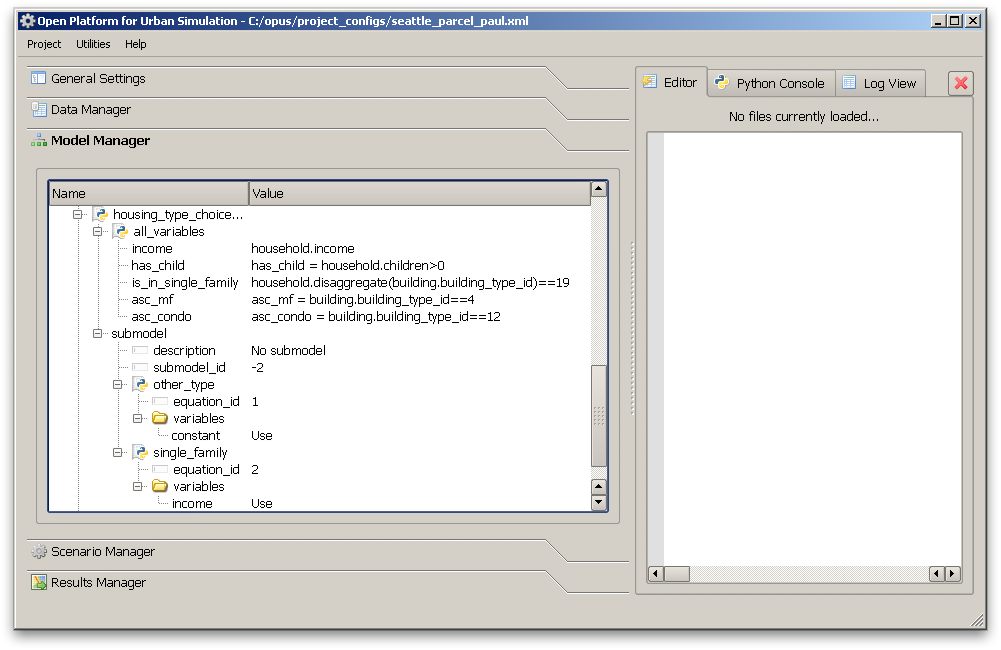
\includegraphics[scale=0.35]{graphics/choice-model-specification.png}
%\end{center}
%\caption{Specifying the Housing Type Choice Model}
%\label{fig:choice-model-specification}
%\end{figure}

%\begin{figure}[htp]
%\begin{center}
%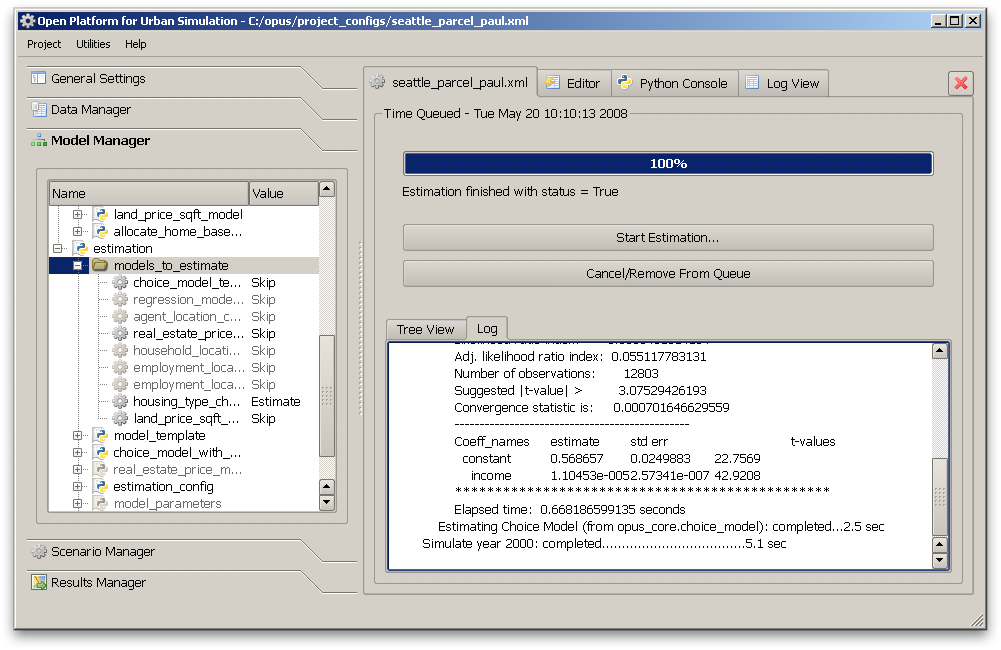
\includegraphics[scale=0.35]{graphics/choice-model-estimation.png}
%\end{center}
%\caption{Estimating the Housing Type Choice Model}
%\label{fig:choice-model-estimation}
%\end{figure}

\chapter{The Scenarios Manager}
\label{chap:scenarios-manager}

\section{Running a Simulation}
Once a project has been developed, including the data to be used in it, and the model system has been configured and the parameters for the models estimated, the next step is to create and run a scenario.  In the eugene\_gridcell project, a baseline scenario has already been created and is ready to run.  To run this scenario, in the Scenario Manager, right-click with the mouse on the Eugene-baseline entry and select \verb#Run this Scenario#.  At this point, a frame should appear in the right hand side of the Opus window, as shown in Figure \ref{fig:opus-start-run}.

\begin{figure}[htp]
\begin{center}
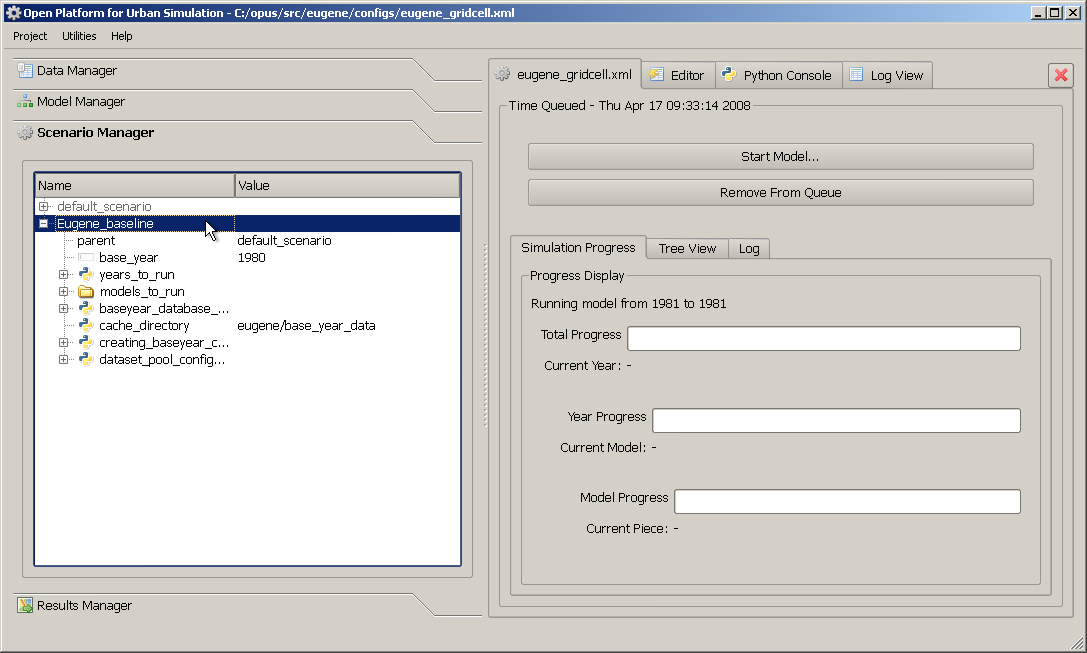
\includegraphics[scale=0.4]{graphics/opus-start-run.png}
\end{center}
\caption{Starting a Simulation on a Scenario.xml}
\label{fig:opus-start-run}
\end{figure}

The frame on the right contains an option to start the run and an
option to remove the run from the queue.  The latter will remove this
new frame so that it is no longer available to run.  Start the run with
the first button option, labelled \verb#Start Model#.  The window will
now update as the simulation proceeds, with progress bars and labels
being updated to show the changing state of the system, such as what
year the model is simulating, what model is running, and even what part
of a model is running.  Figure \ref{fig:opus-running} shows the updated
window in this state.  Note that the \verb#Start Model#  button label
has now changed to \verb#Pause Model#.  If this is pressed while the
model system is running, a request to pause the model is triggered, and
once the current model in the model system is finished, the system
pauses until you take further action, like resume, or remove from
queue.

\begin{figure}[htp]
\begin{center}
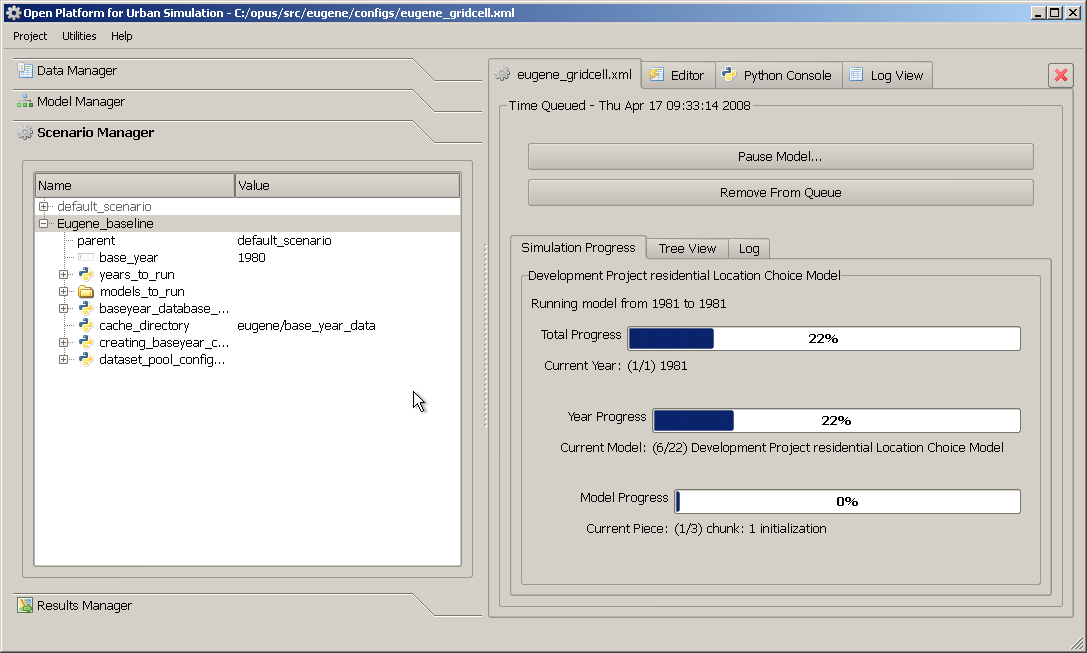
\includegraphics[scale=0.4]{graphics/opus-running.png}
\end{center}
\caption{Running a Simulation on a Scenario.xml}
\label{fig:opus-running}
\end{figure}


% \begin{figure}[htp]
% \begin{center}
% 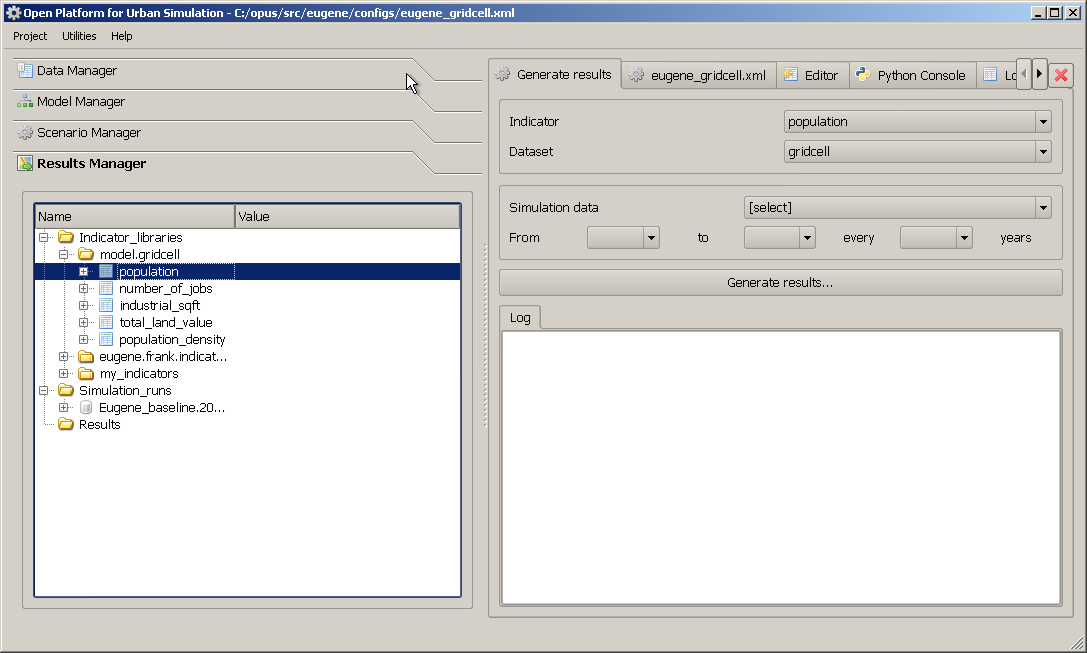
\includegraphics[scale=0.4]{graphics/opus-generate-indicator.png}
% \end{center}
% \caption{Generating an Indicator in the Results Manager}
% \label{fig:opus-generate-indicator}
% \end{figure}


\chapter{The Results Manager}

The Results Manager, corresponding to the Results tab of the GUI, has
two main responsibilities: to manage simulation runs for this project
and to allow the interrogation of these simulation results through
the use of \emph{indicators}. We explore both of these in this
chapter.

\section{Managing simulation runs}

[get run info]
[remove run and delete from harddrive]
[import run from disk]


\section{Interrogating results with Indicators}

Indicators are variables defined explicitly
for use as a meaningful measure. Like model variables, they can be
defined using the domain-specific programming language via the
``Variable Library'' item in the Tools menu. (XXX: forward pointer to
indicator chapter). An indicator can then be visualized as either a
map or as a table (the raw data) in a variety of formats. 

The GUI provides two ways to use indicators to understand what has
happened in your simulation:
\begin{enumerate}
  \item Interactive result exploration
  \item Batch indicator configuration and execution
\end{enumerate} 

\subsection{Interactive result exploration}

Often, it is desirable to explore your results in a lightweight
fashion in order to get a basic idea of what happened. You don't
necessarily want to go through the process of exporting results to a
GIS mapping tool in order to gain some intuition. 

The Opus GUI's \verb#Result Browser#, available from the \verb#tools#
menu, allows interactive exploration of simulation results. The Result
Browser presents a selectable list of available simulation runs, years
over which those simulations were run, and available indicators. You
can then configure an indicator visualization by selecting a simulation
run, a year, and an indicator. To compute and visualize the configured
indicator, simply press the \verb#generate results# button. The
indicator will then be computed for the year of the selected simulation
run. After it is computed, a tab should appear at the bottom of the
window with the name of the indicator and provide the ability to
visualize the results as a table or map (using the MatplotLib Python
module). See the inset tutorial XXX to try out the \verb#Result
Browser#.

\fbox{
\begin{minipage}{.5\linewidth}
\begin{enumerate}
  \item \cmd{Open the Results Browser from the Tools menu. Use the
  Results Browser to answer the following questions.}
  \item \question{Just from visual inspection, is there more than one
  cluster of gridcells with high land value in the Eugene region in 1980 in the baseyear data?}
  \item \question{Is this cluster(s) in the same general area as the
  greatest number of jobs in Eugene for the same year of the
  baseyear data?}
\end{enumerate}
\end{minipage}
}

Two additional aspects of the Result Browser should be mentioned:
\begin{enumerate}
  \item If the checkbox \verb#Automatically view indicator# is
  clicked, everytime you change the indicator configuration (i.e.
  select a different simulation run, year, or indicator), the
  indicator will be automatically visualized (as if you pressed the
  \verb#Generate results# button). 
  \item The \verb#Export results# button will export the table data
  of the currently configured indicator to a database. This feature
  is not yet implemented. 
\end{enumerate}

\subsection{Batch indicator configuration and execution}

The \verb#Result Browser# is good for poking around in the
data. But often you'll want to generate the same
set of indicators for each of amny runs and you don't want to
redefine them every time. Instead, you'd like to configure and save a
group of them that can be executed on demand on an arbitrary
simulation run. In the Opus GUI, this functionality is supported with
\emph{indicator batches}. 

To create a new indicator batch, right-click on the
\verb#Indicator_batches# node in the \verb#Results tab# and select
\verb#Add new indicator batch...#. A new batch will be created
under the Indicator_batches node. You can rename the new batch if you
want by double-clicking its name and typing in a new one.

A batch is a collection of \verb#Indicator visualization#
definitions. Each indicator visualization is a configuration of
the indicator variable to be used, a visualization style (e.g. map or
table), and some format options. To add a new indicator visualization
to the batch, right-click on the respective batch and select
\verb#Add new indicator visualization...#. A dialog box will
appear where you can define the visualization. The visualization
options for an indicator visualzation are discussed in depth later in
subsection~\ref{sect:indicator_visualization_options}.

You can add as many indicator visualizations to a batch as you want.
In order to execute an indicator batch on a simulation run,
right-click on the indicator batch and hover over \verb#Run indicator
batch on...#. A list of all the available simulations runs will
appear as a submenu. You can then select the appropriate simulation
and the indicator visualizations in the batch will be executed over
all the years of that simulation run. If the resulting indicators are
tables or maps stored in a file, they can then be found on disk in
your \verb#OPUSHOME/data/PROJECTNAME/runs/RUNNAME/indicators#
directory, where \verb#PROJECTNAME# is the name of your project (e.g.
``eugene\_gridcell'') and \verb#RUNNAME# is the name of the
simulation run that you selected to run the batch on. The indicator
visualizations configured to write to a database will have produced
tables in the specified database with the name of the respective
indicator visualization. 


\subsubsection{Indicator visualization configuration options}
\label{sect:indicator_visualization_options}

Opus provides a rich variety of ways to visualize indicators and this
functionality is exposed in the \verb#Indicator visualization# dialog
box options (e.g. multi-year indicators, exporting to
databases). Unfortunately, this functionality can sometimes be hard
to present in an intuitive fashion. This section describes the range
of available options in the Batch indicator visualization dialog
box, which is separated into three components: ``indicator
selection'', ``output options'', and ``format options''. 

{\bf Indicator selection}

The bottom of the dialog box has two list boxes, ``available
indicators'' and ``indicators in current visualization''. The
indicators here are those variables from the \verb#Variable Library#
(XXX reference to variable library section) whose \emph{use} has been
set to be \emph{indicator} or \emph{both}. Note that the set of
indicators available is filtered by the currently selected dataset in
the ``output options'' (described later in this section).

By moving an indicator from the ``available indicators'' box to the
``indicators in current visualization'' box via the ``+'' button, you
include that indicator in this indicator visualization. Likewise, to
remove an indicator from the visualization, select the indicator in
the ``indicators in current visualization'' box and press the ``-''
button.


{\bf Output options}

\emph{Visualization Name}. The base name of any produced
visualizations. Because you might be producing this visualization for
different years and different simulation data, more information wil
be appended to this name to ensure uniqueness of the resulting file
or database table when the visualization is run on some data. 

\emph{Type}. There are two different types of indicator
visualizations that can be produced: maps and tables. Tables are just
raw data organized into rows and columns, while maps are
spatial projections of this data. The available format options
(described later) are fully dependent on the visualization type. 

\emph{Dataset name}. The dataset that this visualization corresponds
to. When the selected indicator(s) are run, they will be computed over
this dataset. Most commonly you are choosing a geographic granularity
(e.g. gridcell, zone) that you want to see the results at. Note that
when you change the dataset, the set of available indicators changes
because a given indicator is valid only for a single dataset.

{\bf Format options for maps}

The Matplotlib map is not intended to replace GIS-based mapping, which
allows far more control and the overlay of other features for visual
reference.  It is merely a quick tool to visualize data to get a sense
of the spatial patterns in it.  In order to support visualization in a
GIS environment such as ArcGIS or QGIS, the results may be exported to
a database or geodatabase environment, and the GIS software used to
create a more interactive and flexible display of the data.


{\bf Format options for tables}


[export results to database; geodatabase / autoview creation in
Postgres]



% 
% \subsection{Generating Indicators}
% 
% 
% 
% You will need to click the \verb#Simulation data# button and then
% select the simulation results you want to use.  Notice that the name of
% the scenario contains a date and time when the run was started.  Once
% you click on the \verb#Generate results# button, the indicator is
% computed.  A message is printed to the log, below the button, and a new
% entry will show up in the results node in the Results Manager tab on
% the left, as shown in Figure \ref{fig:opus-indicator-2}.
% 
% \begin{figure}[htp]
% \begin{center}
% 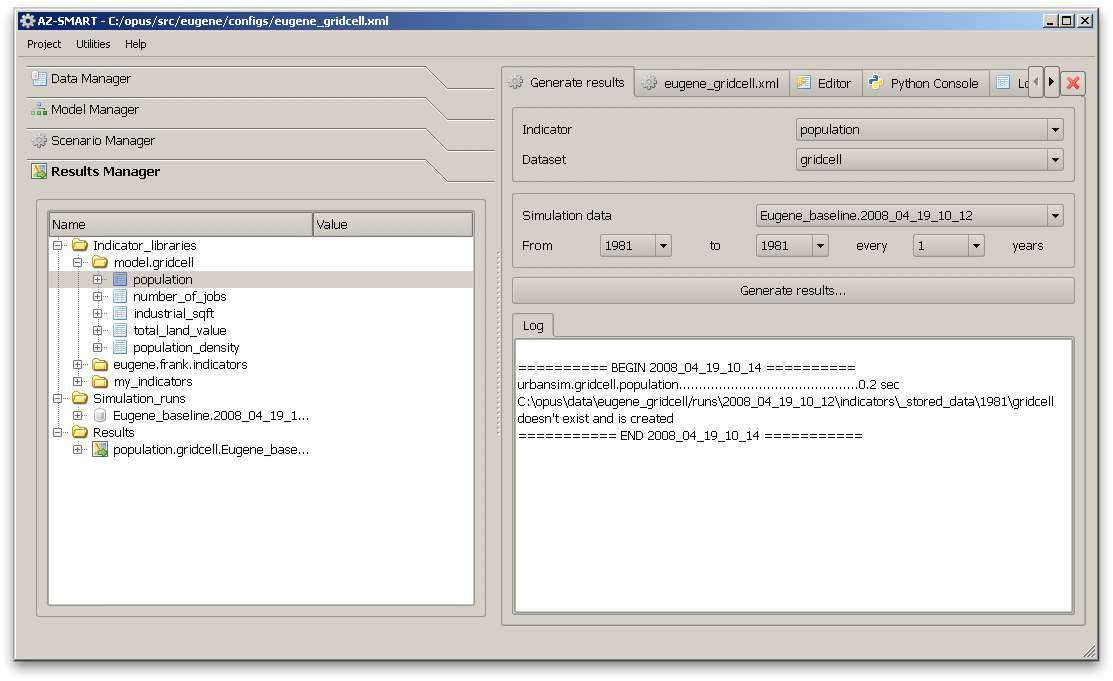
\includegraphics[scale=0.4]{graphics/opus-indicator-2.png}
% \end{center}
% \caption{Result of Generating an Indicator}
% \label{fig:opus-indicator-2}
% \end{figure}
% 
% Now that an indicator has been computed, its data is available to
% visualize or export to another application.  The Results Manager
% currently supports several ways to visualize an indicator, and these
% will depend on the nature of the indicator.  The menu for this is shown
% in Figure \ref{fig:opus-indicator-view-1}.  For example, the indicator
% that has just been computed is population by gridcell.  It is possible
% to visualize data on a grid using a simple image map, displayed on the
% right hand window using the Matplotlib Python library.   If you select
% the Map (Matplotlib) option on the menu, it will generate a map such as
% the one shown in Figure \ref{fig:opus-indicator-view-2}.
% 
% \begin{figure}[htp]
% \begin{center}
% 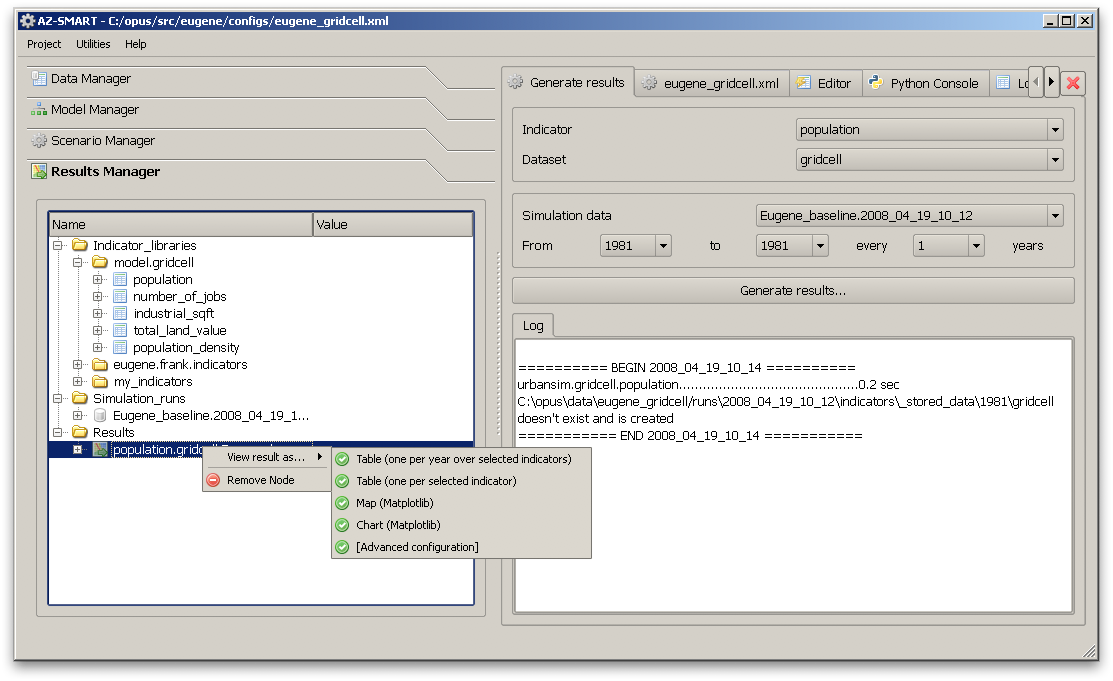
\includegraphics[scale=0.4]{graphics/opus-indicator-view-1.png}
% \end{center}
% \caption{View Results for an Indicator}
% \label{fig:opus-indicator-view-1}
% \end{figure}
% 
% \begin{figure}[htp]
% \begin{center}
% 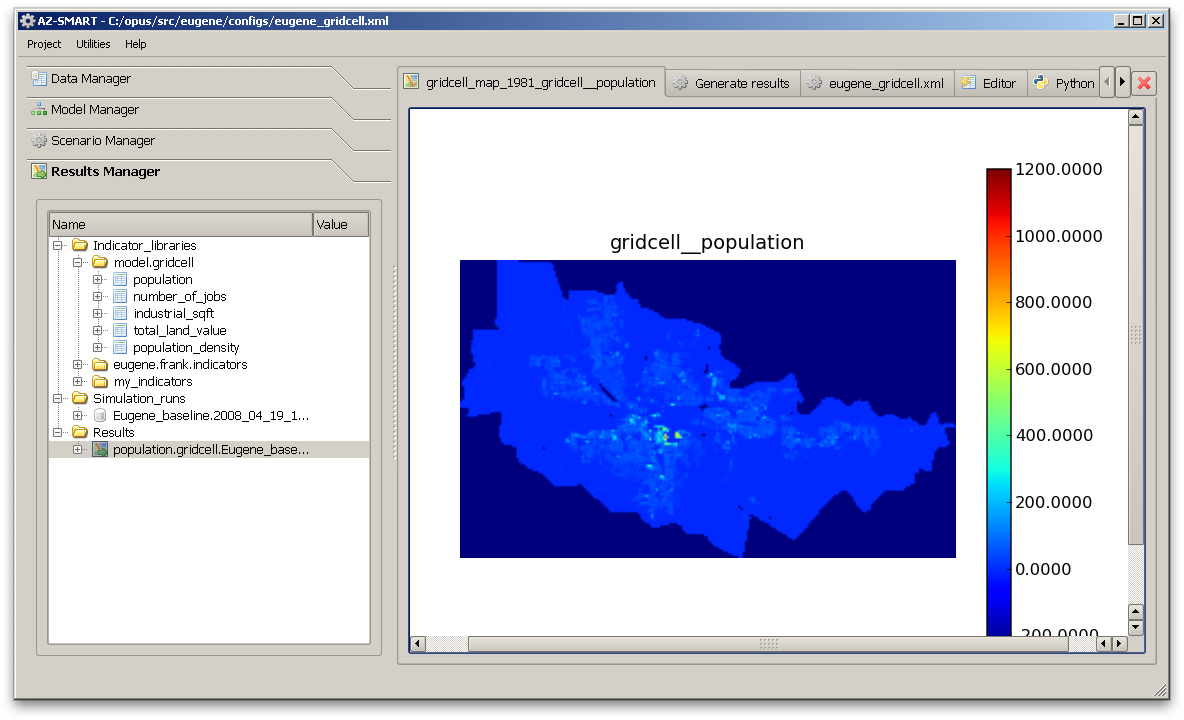
\includegraphics[scale=0.4]{graphics/opus-indicator-view-2.png}
% \end{center}
% \caption{Matplotlib Map for Population by Gridcell in Eugene-Springfield in 1981}
% \label{fig:opus-indicator-view-2}
% \end{figure}
% 
% The Matplotlib map is not intended to replace GIS-based mapping, which
% allows far more control and the overlay of other features for visual
% reference.  It is merely a quick tool to visualize data to get a sense
% of the spatial patterns in it.  In order to support visualization in a
% GIS environment such as ArcGIS or QGIS, the results may be exported to
% a database or geodatabase environment, and the GIS software used to
% create a more interactive and flexible display of the data.
% 

\chapter{XML-based Project Configurations and Inheritance}
\label{chapter:xml-inheritance}

As previously discussed, Opus uses XML-based configuration files to
flexibly specify the various aspects of a project as well as to specify the
appearance of the different tabs in the GUI\@.

One configuration (the \emph{child}) can inherit from another configuration
(the \emph{parent}).  By default, the child inherits all the information
contained in the project.  However, it can override any information
inherited from the parent, and add additional information.  This means that
you can use default projects as parents for another project you want to
create that is mostly the same as an existing project, but has some changes
from it.  An XML configuration specifies its parent using the \emph{parent}
entry under the ``General'' section of the XML\@.  The value of this is the
name of the XML file that contains the parent configuration.  When
searching for this file, Opus first looks in the same directory that holds
the child configuration.  If it's not found there, it expects to find a
path in the Opus source code tree, starting with the name of a project like
\package{eugene} or \package{urbansim}.

This works well with the convention that users should create their own
projects in the \file{opus/project_configs} directory.  You can have
several configurations in your \file{opus/project_configs} directory, one
inheriting from the other.  Ultimately, though, one or more of these
configurations should inherit from a default configuration in the source
tree.  For example, Figure \ref{fig:eugene-gridcell-xml-default} shows the
contents of the default project for \file{eugene_gridcell} in
\file{opus/project_configs}.  This has almost no content of its own, but
rather inherits almost everything from the default configuration in the
source tree at \file{eugene/configs/eugene_gridcell.xml}.

\begin{figure}[htp]
\begin{center}
\begin{verbatim}
<opus_project>
  <general>
    <description type="string">Minimal user configuration for the Eugene 
        gridcell project</description>
    <parent type="file">eugene/configs/eugene_gridcell.xml</parent>
  </general>
</opus_project>
\end{verbatim}
\end{center}
\caption{Contents of the default eugene\_gridcell.xml project}
\label{fig:eugene-gridcell-xml-default}
\end{figure}

A small section of the \file{eugene/configs/eugene_gridcell.xml} file is
shown in Figure \ref{fig:opus-xml}.  It is just text, but in a structured
format, with nodes corresponding to information that is displayed in the
GUI.  Some of the content of the XML provide data used by the GUI to
determine how to display information, or what menu items are appropriate to
connect to the node in the GUI.  Notice that this project in turn inherits
from \file{urbansim_gridcell/configs/urbansim_gridcell.xml}.

\begin{figure}[htp]
\begin{center}
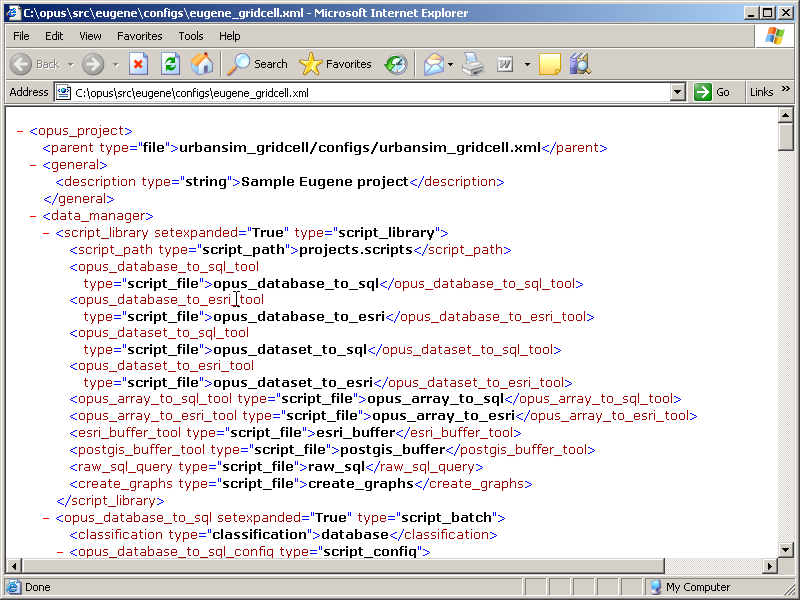
\includegraphics[scale=0.4]{graphics/opus-xml.png}
\end{center}
\caption{An Excerpt from eugene/configs/eugene\_gridcell.xml}
\label{fig:opus-xml}
\end{figure}

To change any of the options in the XML tree you need to be able to edit
it.  Inherited parts of the XML tree are shown in blue in the left pane in
the GUI\@.  These can't be edited directly --- they just show inherited
information.  You can make an inherited portion of the XML tree editable by
right clicking on it and selecting `Add to curent project.''  This copies
the inherited information into the local XML tree.  (We saw an example of
doing this in Section \ref{sec:configuring-scenario}.)

A few details about the ``Add to current project'' command: in Section
\ref{sec:configuring-scenario}, when we added \code{lastyear} to the
current project, the containing nodes in the tree (\code{years_to_run} and
\code{Eugene_baseline}) also turned black, since they needed to be added to
the current project as well to hold \code{lastyear}.  It's also possible to
click directly on \code{years_to_run}, or even \code{Eugene_baseline}, and
add the XML tree under that to the current project.  However, we recommend
adding just the part you're editing to the current project, and not others.
(You can always add other parts later.)  The reason is that once a part of
the tree is added to the current project, the inheritance relation of that
part with the parent disappears, and changes to the parent won't be
reflected in the child XML\@.  For example, if you add all of the
\code{Eugene_baseline} node to the current project, save your
configuration, and then update the source code, changes to some obscure
advanced feature in the XML in the parent in the source tree wouldn't show
up in your configuration.

